%----------------------------------------------------------------------------------------
%	PACKAGES AND OTHER DOCUMENT CONFIGURATIONS
%----------------------------------------------------------------------------------------

\documentclass[12pt]{article}
\usepackage[danish]{babel}
\usepackage[numbered,final]{mcode}
\usepackage[utf8x]{inputenc}
\usepackage{amsmath}
\usepackage{graphicx}
\usepackage[colorinlistoftodos]{todonotes}
\usepackage[toc,page]{appendix}
%\usepackage{float}
\usepackage{floatrow} % used for adding "Source" to pictures
\usepackage{hyperref} % used for hyperlinks
\usepackage[all]{hypcap}
\usepackage{bm} % used for bold inline matj
\usepackage{lipsum} % used for lorem lipsum
\usepackage[final]{pdfpages} % used for including PDF's
\usepackage{geometry}
\usepackage{listingsutf8}
\usepackage{listings}
\usepackage{color} %red, green, blue, yellow, cyan, magenta, black, white
\definecolor{mygreen}{RGB}{28,172,0} % color values Red, Green, Blue
\definecolor{mylilas}{RGB}{170,55,241}

\hypersetup{colorlinks=true, linkcolor=black}

% Page margins
\geometry{verbose,tmargin=1in,bmargin=1in,lmargin=1in,rmargin=1in,headsep=0.35in}


\begin{document}

\begin{titlepage}



\newcommand{\HRule}{\rule{\linewidth}{0.5mm}} % Defines a new command for the horizontal lines, change thickness here
\setlength{\topmargin}{0in}
\centering % Center everything on the page

%----------------------------------------------------------------------------------------
%	HEADING SECTIONS
%----------------------------------------------------------------------------------------
\textsc{\LARGE Aarhus universitet}\\[1.5cm] % Name of your university/college
\textsc{\Large Introduktion til digital signalbehandling}\\[0.5cm] % Major heading such as course name
\textsc{\large 3. Semester}\\[0.5cm] % Minor heading such as course title

%----------------------------------------------------------------------------------------
%	TITLE SECTION
%----------------------------------------------------------------------------------------

\HRule \\[0.4cm]
{ \huge \bfseries DSA Case 2}\\ % Title of your document
\HRule \\[1cm]
 
%----------------------------------------------------------------------------------------
%	AUTHOR SECTION
%----------------------------------------------------------------------------------------

\begin{minipage}{0.4\textwidth}
	\begin{flushleft} \large
		\emph{Gruppemedlemmer:}\\
		Gustav A. Gammelgaard \\
		Stinus Lykke Skovgaard \\
		Tim Hede Stenholt \\ [0.5cm]
	\end{flushleft}
\end{minipage}
~
\begin{minipage}{0.4\textwidth}
	\begin{flushright} \large
		\emph{AUid:} \\
		au538293\\
		au520659\\
		au543518\\ [0.5cm]
	\end{flushright}
\end{minipage}\\[5cm]

%----------------------------------------------------------------------------------------
%	LOGO SECTION
%----------------------------------------------------------------------------------------


\includegraphics[scale=0.5]{Img/logo.jpg}\\[1cm]

%----------------------------------------------------------------------------------------
%	DATE SECTION
%----------------------------------------------------------------------------------------

{\large \today}\\[0.5cm] % Date, change the \today to a set date if you want to be precise


\vfill % Fill the rest of the page with whitespace

\end{titlepage}

\newpage
\tableofcontents
\newpage
\listoffigures
\newpage

\hypersetup{linkcolor=blue}

\section{Problem beskrivelse}
\begin{flushleft}
		Denne case omhandler måden at forbedre et støjfyldt signal med et midlingsfilter. Dette filter skal midle et signal fra en vægt. Typisk vil signalet fra vægten svinge voldsomt som vil gøre det svært at måle korrekt. Midlingsfilteret vil gøre det muligt at få en pålidelig måling. Filteret er realiseret ved hjælp af matlab og vægt data er importeret ind i matlab og testet i dette miljø.
\end{flushleft}

\section{Opgave 1 - Data analyse}
Ved data analysen er det udleverede materiale blevet plottet som en sample tidsakse. Dette viser at vores signal har et område med og uden vægt på. 

\begin{figure}[H]
	\centering
	\includegraphics[width=90mm]{Img/sample_akse.png}
	\caption{Sample akse for hele signalet}
	% \floatfoot{Source: (Citation command)}
	\label{fig:sample_akse}
\end{figure}

på figur \ref{fig:sample_akse} kan mas se den belastede og ubelasede del af signalet. Da dataen skal bruges i et midlingsfilter undlader vi at bruge de samples der ligger i ændringen, da signalet først skal falde til ro. Derfor får vi to signaler der bliver kørt filtre på. Henholdsvis et load signal og noload signal. \\
Hvis dataen fra load og unload signalet plottes på et histogram kan man se hvordan dataen er normalfordelt. Hvis man udregner varians og spredning, får vi spredningen til ca 30. Det passer fint overens med histogrammerne.

\begin{lstlisting}[frame=single]  % Start your code-block
for i:=maxint to 0 do
%Varians
noload_var = (1/size(noload,2))*sum((noload-noload_avg).^2);
load_var = (1/size(load,2))*sum((load-load_avg).^2);

%Spredning
noload_spred = sqrt(noload_var);
load_spred = sqrt(load_var);
\end{lstlisting}

Dette passer fint overens med histogrammerne på figur \ref{fig:histogram1} og \ref{fig:histogram2}.

Hvis vi plotter load og noload i effekt-spektret kan man se at det ligner hvid støj, dog med en enkelt spike ved DC.

\begin{figure}[H]
	\centering
	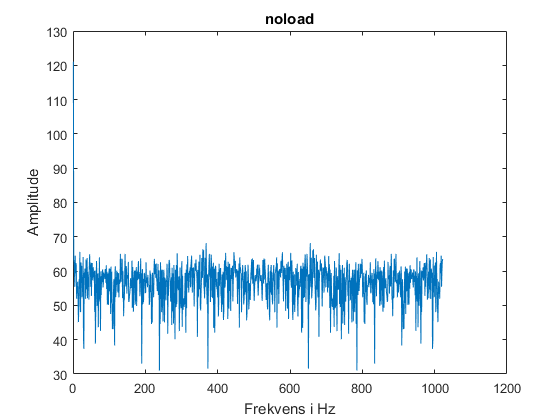
\includegraphics[width=90mm]{Img/noload_effekt.png}
	\caption{Effekt-spektrum for noload}
	% \floatfoot{Source: (Citation command)}
	\label{fig:effekt_noload}
\end{figure}

\begin{figure}[H]
	\centering
	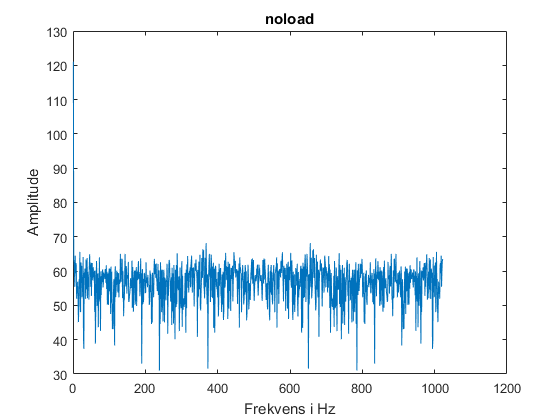
\includegraphics[width=90mm]{Img/noload_effekt.png}
	\caption{Effekt-spektrum for load}
	% \floatfoot{Source: (Citation command)}
	\label{fig:effekt_load}
\end{figure}

For at finde afstenden mellem hver bit-niveau i gram, laver vi følgenede udregning.

\begin{lstlisting}[frame=single]  % Start your code-block
for i:=maxint to 0 do
LSB_value = 1000/valueDiff
\end{lstlisting}

Dette giver os en LSB værdi på 3.3.

\section{Opgave 2 - Design af midlingsfilter}
Det kommende afsnit kommer til at omhandle hvordan midlingsfilteret virker og hvordan det er implementeret. Filteret er blevet testet på dataen fra opgave 1. Vi har ekspermenteret med både lineært og eksponentielt midlingsfilter. 

\subsection{Lineært midlingsfilter}
Det lineære midlingsfilter fungerer ved løbende at tage M inputværdier og dividerer dem med M. Differensligningen for dette ser sådan ud:

\[ y(n)= (1/M)(x(n)+x(n-1)+...+x(n-M+1))\]

Der er en indsvingningstid for filteret, da de første M værdier ikke passer overens med signalet. Det vil sige at de første M samples i filter outputtet bliver lavere. Dette kaldes indsvingningstiden. Dette kan ses på figur \ref{fig:stem_fir}.

\begin{figure}[H]
	\centering
	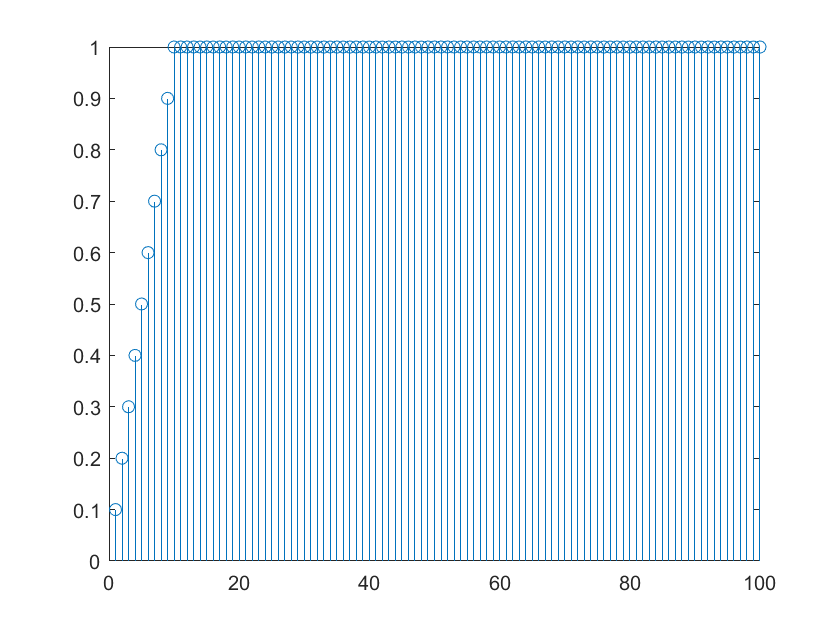
\includegraphics[width=90mm]{Img/respons_alm.png}
	\caption{Histogram af load med og uden filter. Filterorden = 10}
	% \floatfoot{Source: (Citation command)}
	\label{fig:stem_fir}
\end{figure}

For at midle data fra opgave 1, lavede vi først et lineært midlingsfilter. Dette er gjort på følgende måde:

\begin{lstlisting}[frame=single]  % Start your code-block
for i:=maxint to 0 do
M = 10;
h1 = 1/M * ones(1, M);
\end{lstlisting}
Dette laver et midlingsfilter med M koeficienter, der hver har en værdi på 1/M. Ved at indstille på ordnen(altså M) vil man kunne få filteret til midle kraftigere. \\

Da dataen fra opgave 1 viser at der både er en load og noload, er filteret påført de to stadier hver for sig. Dette er blevet plottet på et histogram, som kan ses på figur \ref{fig:histogram1}

\begin{figure}[H]
	\centering
	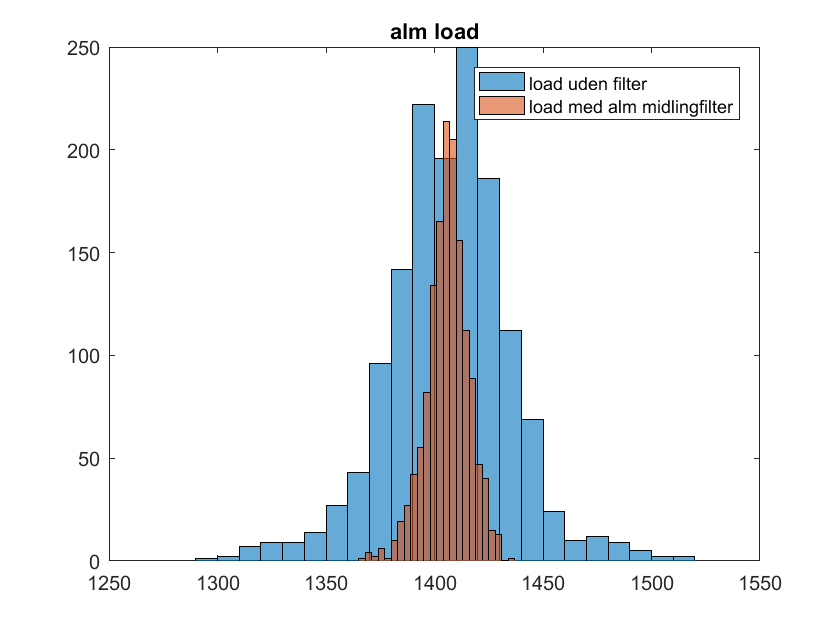
\includegraphics[width=90mm]{Img/Histogram_load_L.png}
	\caption{Filter respons for det lineære midlingsfilter}
	% \floatfoot{Source: (Citation command)}
	\label{fig:histogram1}
\end{figure}

Man kan se at filteret får vores data til at ligge tættere på hinanden, hvilket er det vi gerne vil se. Det samme kan ses for noload på \ref{fig:histogram2}

\begin{figure}[H]
	\centering
	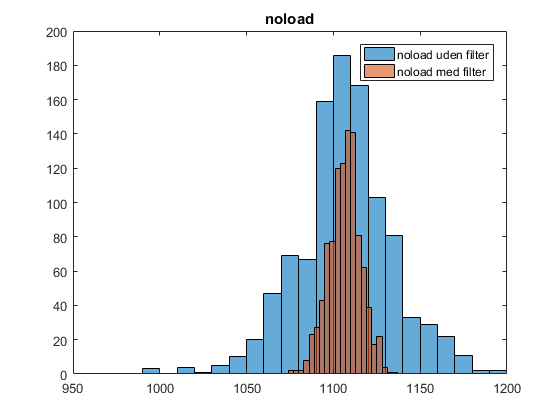
\includegraphics[width=90mm]{Img/Histogram_noload_L.png}
	\caption{Histogram af noload med og uden filter. Filterorden = 10}
	% \floatfoot{Source: (Citation command)}
	\label{fig:histogram2}
\end{figure}

Ved at ændre på ordnen kan man få filtret til at midle kraftigere. Dette kan ses på figur \ref{fig:histogram3}

\begin{figure}[H]
	\centering
	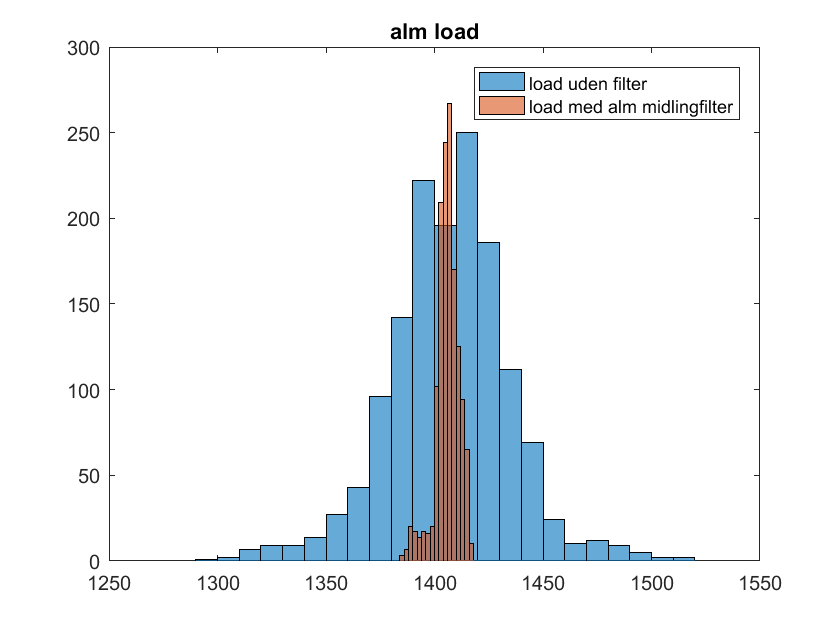
\includegraphics[width=90mm]{Img/Histogram_load_50.png}
	\caption{Histogram af load med og uden filter. Filterorden = 50}
	% \floatfoot{Source: (Citation command)}
	\label{fig:histogram3}
\end{figure}

Det ses tydligt at de orange pinde er blevet smallere og fylder et mindre område på grafen.\\
Hvis man kigger på varians og spredning kan man se at de stemmer godt overens med vores grafer. \\

\begin{lstlisting}[frame=single]  % Start your code-block
for i:=maxint to 0 do

var_load = var(y_load)
var_noload = var(y_noload)

P_load = (1/sqrt(M)*S_load)^2
P_noload = (1/sqrt(M)*S_noload)^2
\end{lstlisting}

Ved M = 10 får vi en varians på ca 90, mod en varians på ca 25 ved en orden på 50. Hvis man kigger på støj-effekten ser man det samme. Ved en orden på 10 er støj-effekten ca 10 højere end ved en orden på 50.\\

Hvis man ønsker en max svingningstid for sit system, bliver man muligvis nødt til at begrænse sin orden på filteret. Hvis vi har et krav om en indsvingningstid på 100ms kan vi lave en hurtigt udregning:

\begin{lstlisting}[frame=single]  % Start your code-block
for i:=maxint to 0 do
maxKoef = fs*0.1;
\end{lstlisting}

Dette giver os et filter med en orden på 30. 
\newpage

\subsection{Eksponentielt midlingsfilter}
Vi forsøgte også at lege med et eksponentielt midlingsfilter. Dette midlingsfilter bruger et
simpelt IIR lavpasfilter beskrevet af differensligningen:
\[ y(n)= \alpha \cdot x(n)+(1-\alpha)\cdot y(n-1) \]
Denne type filter er ofte brugt pga dens fordele, som fx at den kræver færre beregninger per output-sample end et standard midlingsfilter, og dens stærkt reduceret hukommelses brug, idet den kun indeholder et forsinkelse element $y(n-1)$, som skal gemmes i en hukommelsesplads i fx. et embedded system. De nyeste samples $x(n)$ får også størst betydning i outputtet $y(n)$, hvilket betyder at filteret reagerer hurtigere på ændringer i input $x(n)$ et standard midlingsfilter. 
\newline
$\alpha$ er en midlingsfaktor mellem 0 og 1 som bestemmer støjreduktionen i forhold til responstiden. Vi prøvede med en lille værdi af $\alpha$ i vores midlingsfilter, hvilket gav en god støjreduktionen men langsom responstid, omvendt prøvede vi også med en høj værdi af $\alpha$ i vores midlingsfilter, hvilket gav en mindre støjreduktionen, men hurtigere responstid. Så præcis som med det alm midlingsfilter er der et trade off mellem støjreduktionen og responstid.
\newline
$\alpha$ bestemmes ved:
\[ \alpha = \dfrac{2}{R+1} \]
Hvor R er den faktor som støj variensen bliver reduceret. Vi kan sammenligne den eksponentiele midlingsfilters reduktion i støjeffekten direkte med et linært midlingfilters reduktion ved at opskrive:
\[ \alpha = \dfrac{2}{N+1}\]
Hvor N er antal af FIR midlings koeficienter, når $N>3$. Dette har vi prøvet at vise midligning for et eksponentielt midlingsfilter med $N=10$ stemmer nogenlunde med midlingen fra et $N=10$ point linært midlingsfilter fra før. De nye midlinger eksponentielt midlingsfiltere kan ses i \autoref{fig:histogram4} og \autoref{fig:histogram5}

\begin{figure}[H]
	\centering
	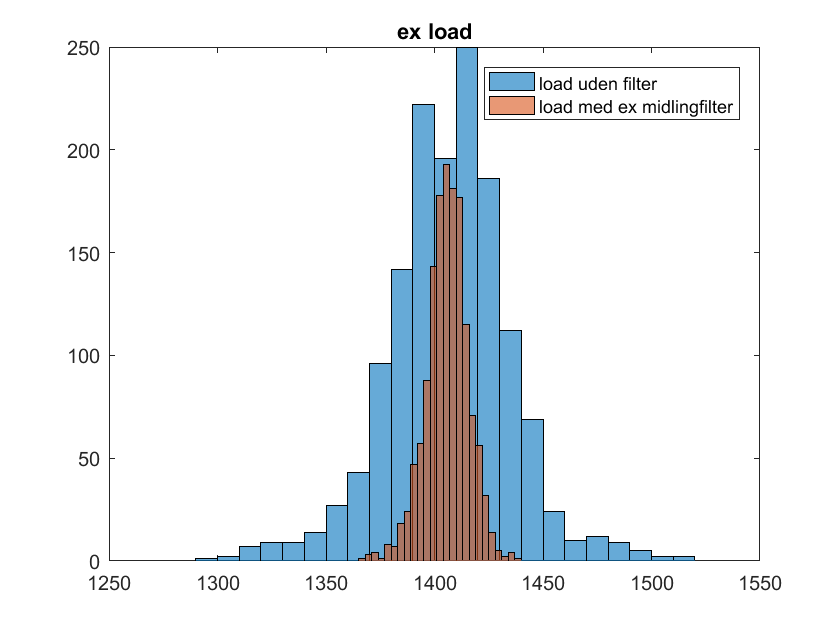
\includegraphics[width=90mm]{Img/Histogram_load_ex10.png}
	\caption{Histogram af load med og uden eksponentielt filter. N = 10}
	% \floatfoot{Source: (Citation command)}
	\label{fig:histogram4}
\end{figure}


\begin{figure}[H]
	\centering
	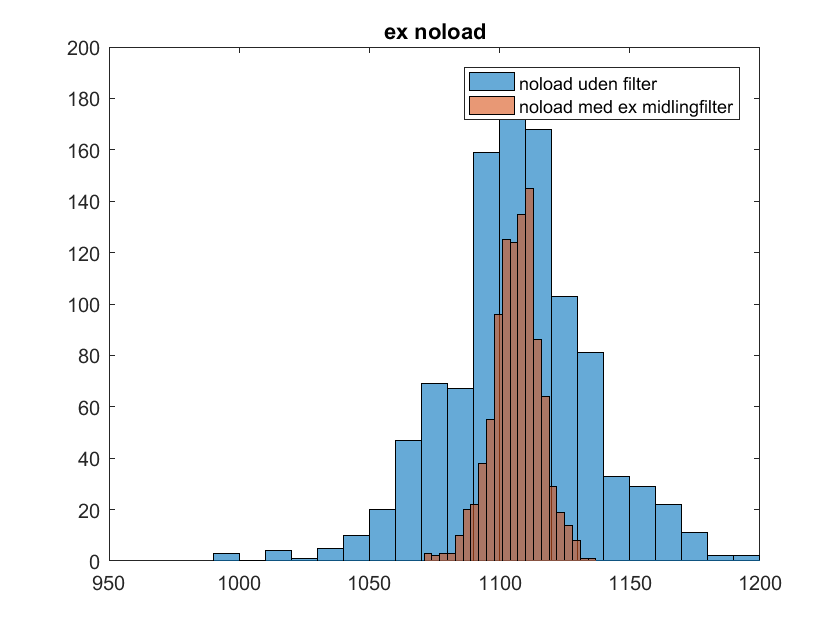
\includegraphics[width=90mm]{Img/Histogram_noload_ex10.png}
	\caption{Histogram af noload med og uden eksponentielt filter. N = 10}
	% \floatfoot{Source: (Citation command)}
	\label{fig:histogram5}
\end{figure}

Som man kan se minder midlingen  for et eksponentielt midlingsfilter i \autoref{fig:histogram4} og \autoref{fig:histogram5} med med midlingen fra de linære midlingsfilter fra før i \autoref{fig:histogram1} og \autoref{fig:histogram2}
\newline
Den store forskel er deres respons på fx. et step som kan ses i \autoref{fig:respons1} og \autoref{fig:respons2}

\begin{figure}[H]
	\centering
	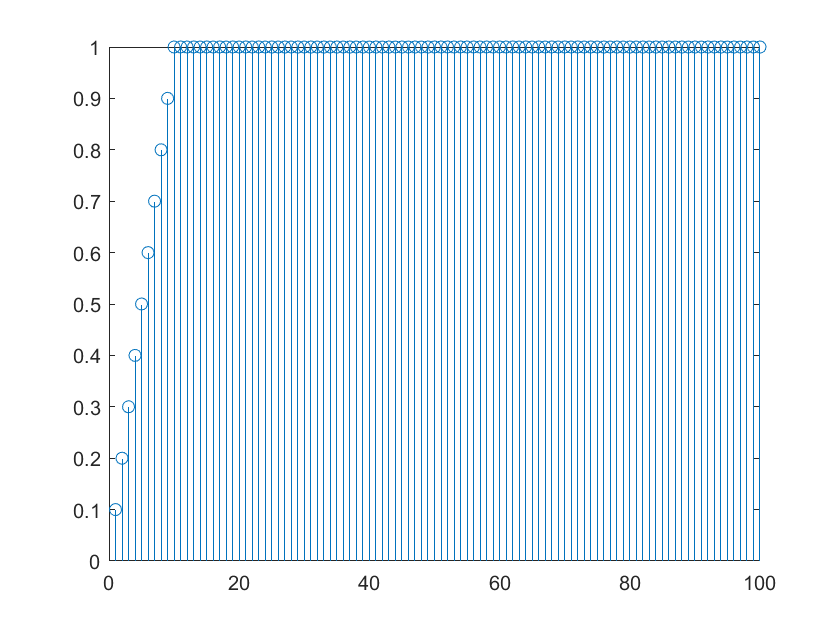
\includegraphics[width=90mm]{Img/respons_alm.png}
	\caption{Linært midlingsfilter respons på step ved M=10.}
	% \floatfoot{Source: (Citation command)}
	\label{fig:respons1}
\end{figure}


\begin{figure}[H]
	\centering
	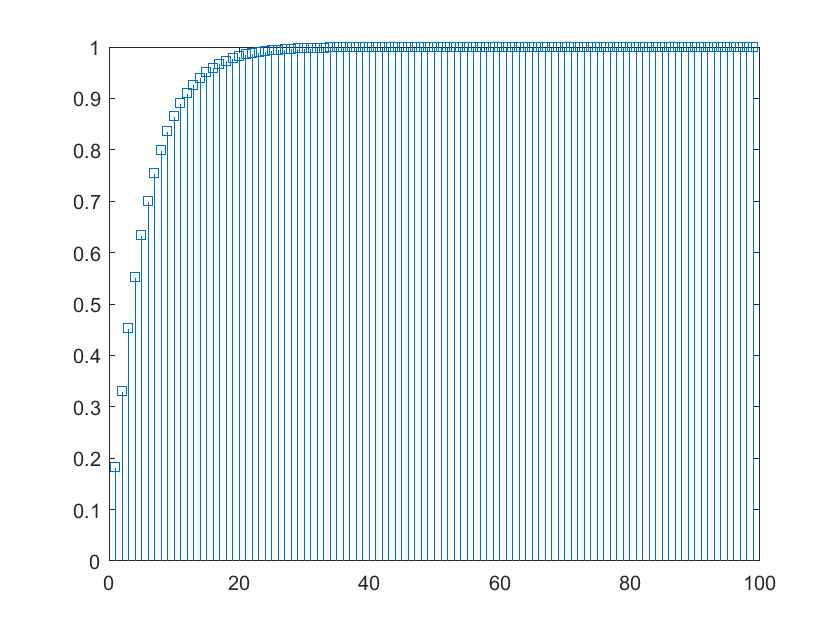
\includegraphics[width=90mm]{Img/respons_ex.png}
	\caption{Ekspontielt midlingsfilter respons på step ved N=10.}
	% \floatfoot{Source: (Citation command)}
	\label{fig:respons2}
\end{figure}
Som det kan ses i \autoref{fig:respons1} og \autoref{fig:respons2}, Så er reagerer det eksponentielle midlingsfilter hurtigere på steppet end det linære midlingsfilter, dog indhentes forspringet fra det eksponentielle midlingsfilter, idet det aldrig kan ramme slutværdien præcis, men blot komme uendelig tæt på. Alligevel tager det ca dobbelt så mange samples for det eksponentielle midlingsfilter at nå til næsten slutværdiden i forhold til det linære filter som når slutværdien efter dens 10 kofficenter er kørt igemme signalet. Dette skyldes at eksponentielle midlingsfilter er et IIR filter som jo har uendeligt respons på et siganal.


\section{Opgave 3 - System overvejelser}

\section{Matlab kode}	

\end{document}